\documentclass[a4paper]{article}
\usepackage[italian]{babel}
\usepackage[utf8]{inputenc}
\usepackage[T1]{fontenc}
\usepackage{graphicx}
\usepackage[export]{adjustbox}
\graphicspath{{./images/}{../cose da aggiungere/pittogrammi/}{../cose da aggiungere/privacy_conformita/}}
\usepackage{caption}
\usepackage{amsmath}
\usepackage{amsfonts}
\usepackage{amssymb}
\usepackage[version=4]{mhchem}
\usepackage{stmaryrd}

\usepackage{float}
\usepackage{tabularx}
\usepackage{array}
\usepackage{fontawesome5}

\usepackage{titling}
\pretitle{\begin{center}
\includegraphics[width=\textwidth]{../cose da aggiungere/header_WATT+}\\[6em]}
	\posttitle{\end{center}}

%\DeclareUnicodeCharacter{00D7}{\ifmmode\times\else{$\times$}\fi}

\title{\Huge{RF-USION POWER+ MANUALE D'USO}}
\date{}

\begin{document}
	
\maketitle

\begin{figure}[H]
	\centering
	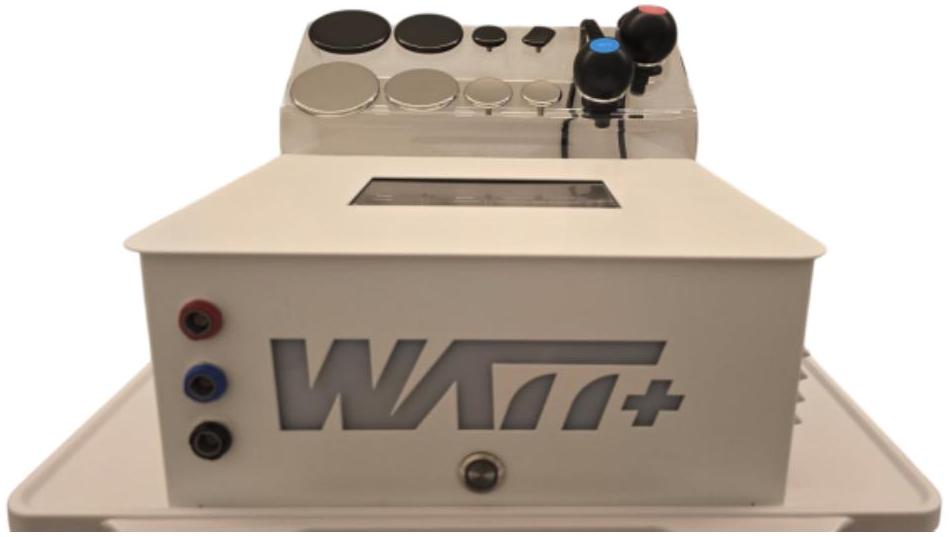
\includegraphics[width=\textwidth]{d37529a0-3e88-4d45-bc8d-f5015b8b0964-01_537_949_475_484}
\end{figure}

\newpage

\tableofcontents

\newpage

\section{Istruzioni di sicurezza}
Per garantire un uso corretto e sicuro di questo prodotto, leggere attentamente le istruzioni prima dell'uso. Seguire tutte le precauzioni di sicurezza!

\section{Simboli}
\begin{figure}[H]
	\centering
	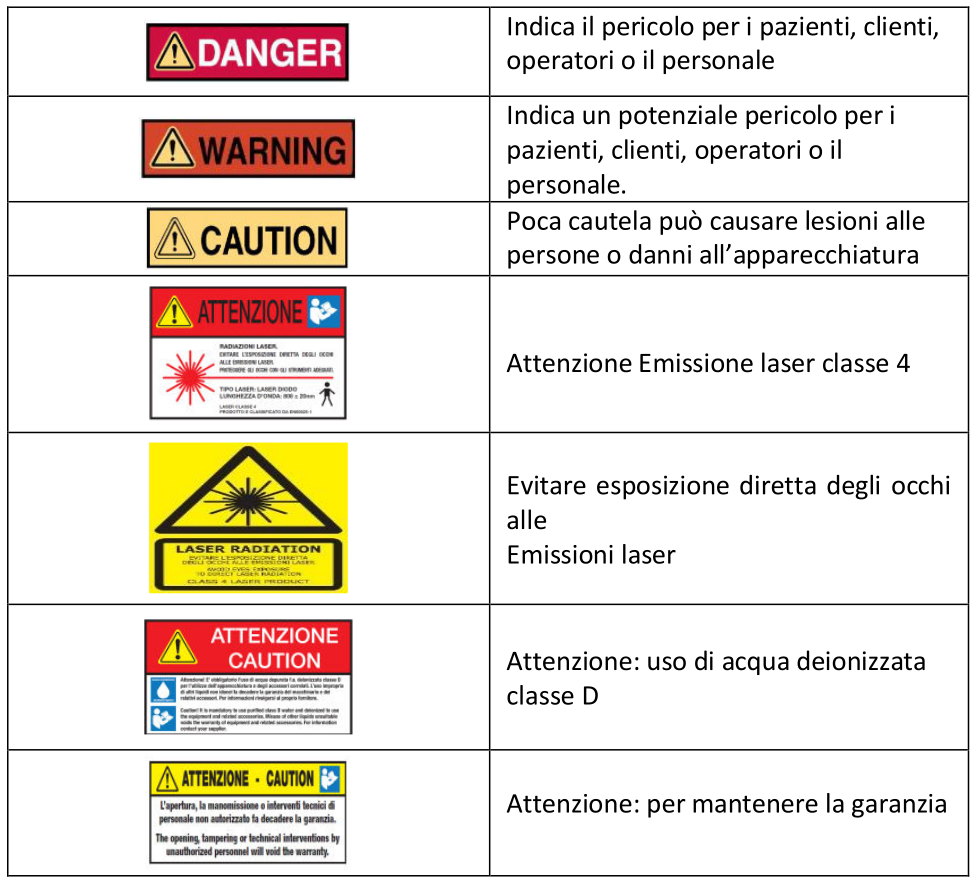
\includegraphics[width=\linewidth]{pittogrammi_1}
%	\caption{}
	\label{fig:pittogrammi1}
\end{figure}
\begin{figure}[H]
	\centering
	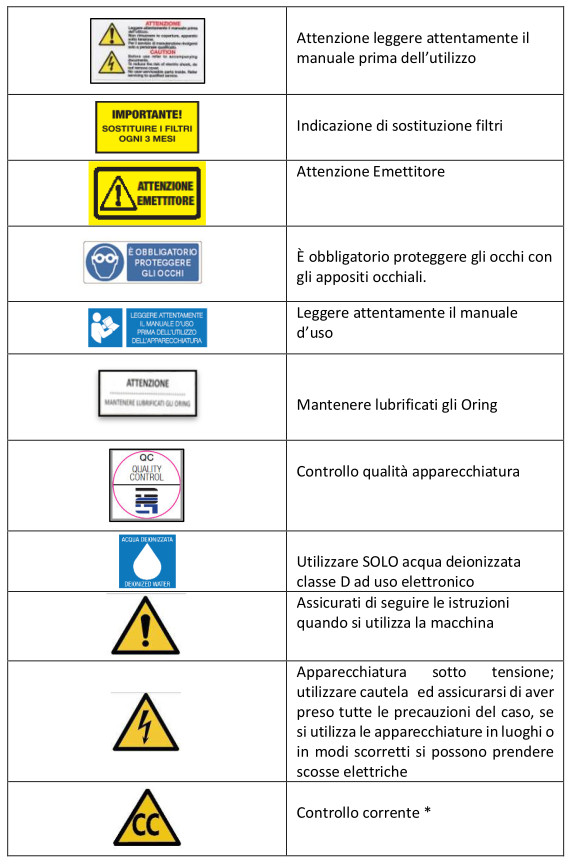
\includegraphics[width=\linewidth]{pittogrammi_2}
%	\caption{}
	\label{fig:pittogrammi2}
\end{figure}
\begin{figure}[H]
	\centering
	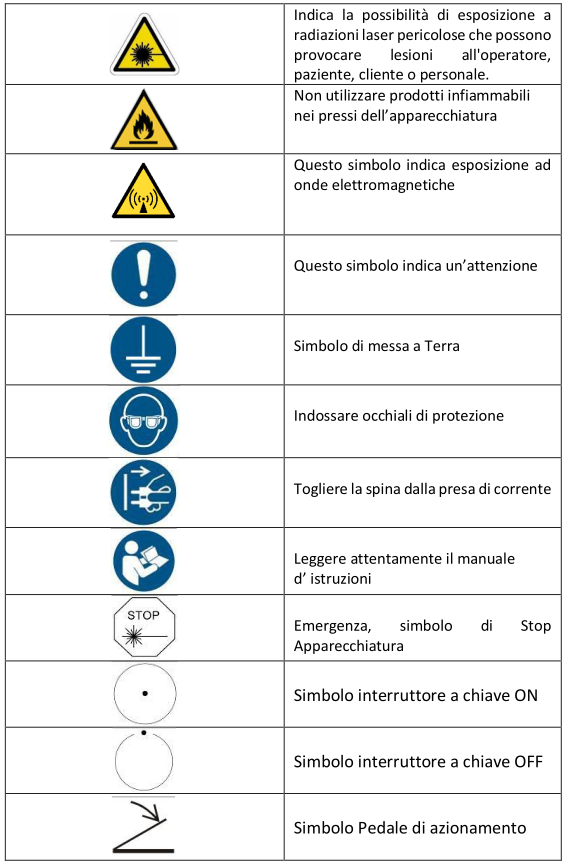
\includegraphics[width=\linewidth]{pittogrammi_3}
%	\caption{}
	\label{fig:pittogrammi3}
\end{figure}
\begin{figure}[H]
	\centering
	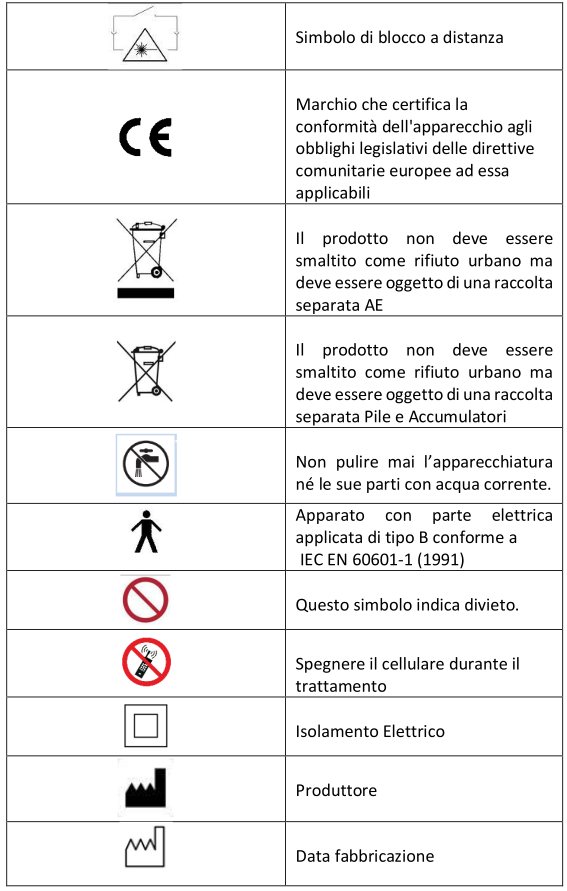
\includegraphics[width=\linewidth]{pittogrammi_4}
%	\caption{}
	\label{fig:pittogrammi4}
\end{figure}
\begin{figure}[H]
	\centering
	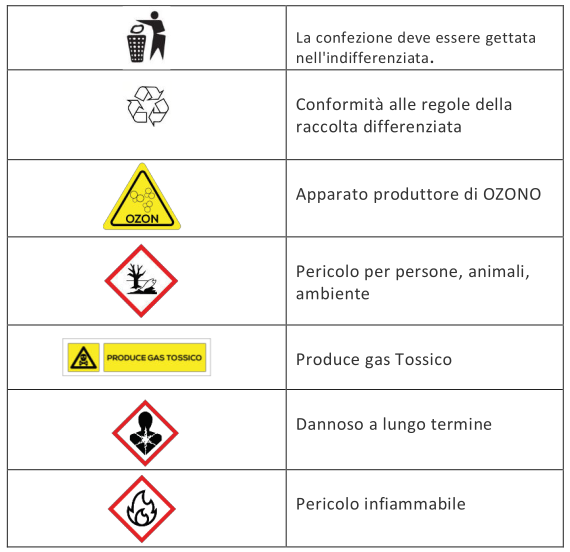
\includegraphics[width=\linewidth]{pittogrammi_5}
%	\caption{}
	\label{fig:pittogrammi5}
\end{figure}


\section{Avvertenze}
Indica una situazione potenzialmente pericolosa che, se non evitata, potrebbe causare gravi perdite di vite umane.

Questo prodotto è destinato esclusivamente a professionisti della bellezza qualificati. Non utilizzarlo o conservarlo in un ambiente umido, come il bagno, per evitare danni e rischi.

Non utilizzare questo prodotto vicino a oggetti infiammabili (ad esempio, alcol, solventi, benzina, solvente per smalto, spray aerosol, ecc.). Non utilizzare questo prodotto nelle seguenti condizioni: quando il cavo di alimentazione o

La spina è danneggiata o calda quando viene staccata dalla presa elettrica. Non usare le mani bagnate per collegare o scollegare i connettori del cavo di alimentazione o per utilizzare questo prodotto.

Assicurarsi che la tensione di esercizio di questo prodotto corrisponda alla tensione nominale.

Avvertimento!

Prima dell'uso, assicurarsi che la spina di alimentazione e il connettore del cavo di alimentazione siano completamente inseriti per evitare situazioni di pericolo.

Quando non è in uso, spegnere il prodotto e scollegarlo.

Pulire regolarmente la polvere accumulata sulla spina e sul connettore del cavo di alimentazione per evitare guasti all'isolamento causati da umidità, polvere e altri fattori.

Non utilizzarlo su altri elettrodomestici.\\
Non avvolgere il cavo di alimentazione attorno al prodotto, poiché ciò potrebbe deformarlo e causare malfunzionamenti.

Tenere fuori dalla portata dei bambini. Non permettere ai bambini di utilizzare questo prodotto.\\
Non modificare, smontare o riparare autonomamente questo prodotto. Se sono necessarie riparazioni, contattare il produttore, un agente o un tecnico di assistenza professionale per l'ispezione e la riparazione, al fine di evitare rischi.

Contattare il distributore, il centro di assistenza o altro personale con competenze ed esperienza adeguate per la riparazione in caso di danni alla spina, poiché ciò potrebbe essere pericoloso. Assicurarsi di utilizzare questo prodotto solo per lo scopo specificato nel presente manuale. Non utilizzare accessori non raccomandati dal produttore.

\section{Attenzione \faExclamationTriangle}
Rappresenta una situazione potenzialmente pericolosa che, se non evitata, potrebbe provocare lesioni personali generali.\\
Gli operatori devono prestare particolare attenzione alla sicurezza del personale e delle attrezzature durante l'uso.\\
Se il prodotto presenta anomalie, interromperne immediatamente l'uso e contattare il produttore o il distributore per un trattamento appropriato.

Questo prodotto e i suoi accessori devono essere maneggiati con cura.\\
Maneggiare correttamente l'imballaggio di questo prodotto per evitare incidenti come il soffocamento dei neonati e tenerlo fuori dalla portata dei bambini.

% manca qualcosa?
\section{Componenti}
\begin{figure}[H]
	\centering
  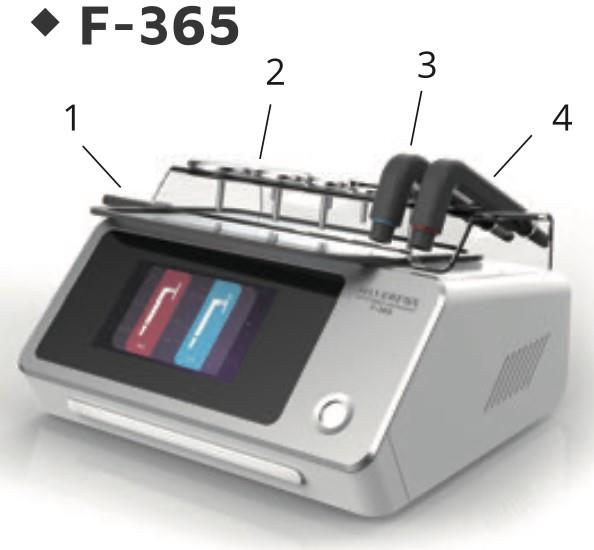
\includegraphics[width=\textwidth]{F-365}
\end{figure}

\begin{enumerate}
	\item 
	Lastra negativa
	\item 
	Elettrodi
	\item 
	Manipolo capacitivo
	\item 
	Manipoli resistivi
\end{enumerate}

%\vspace{20pt}
\newpage

\begin{figure}[H]
	\centering
	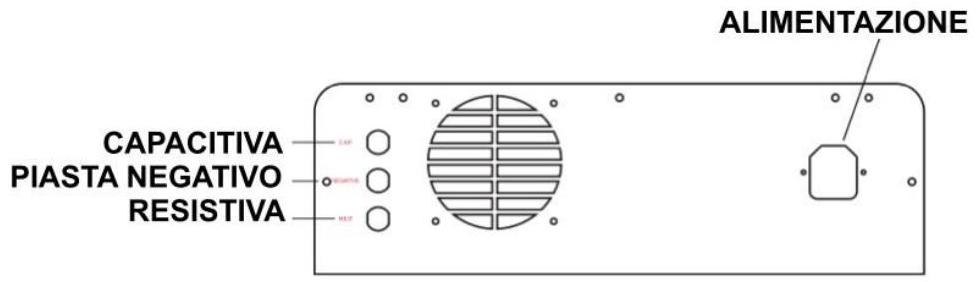
\includegraphics[width=\textwidth]{d37529a0-3e88-4d45-bc8d-f5015b8b0964-03_282_977_1194_529}
  	\captionsetup{labelformat=empty}
	\caption{\textbf{Pannello posteriore}}
\end{figure}


\begin{figure}[H]
	\centering
	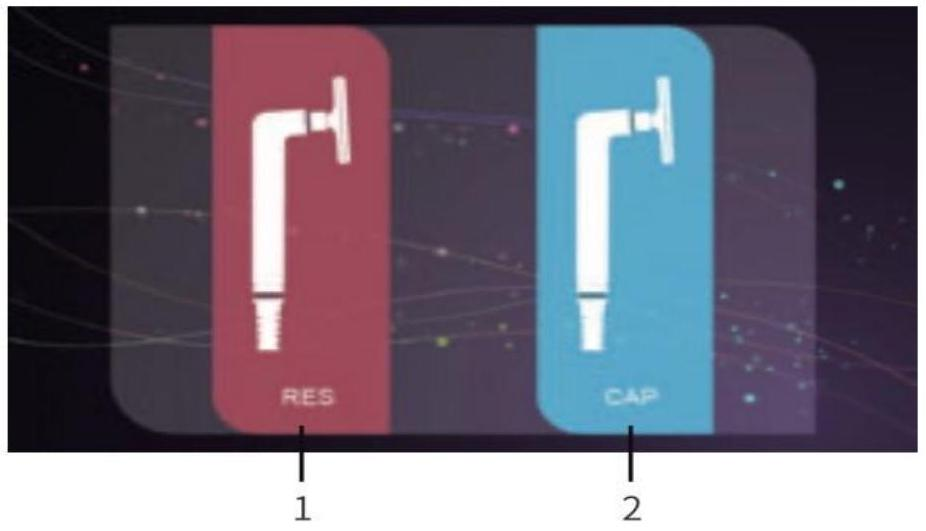
\includegraphics[width=\textwidth]{d37529a0-3e88-4d45-bc8d-f5015b8b0964-03_531_926_2049_571}
	\captionsetup{labelformat=empty}
	\caption{\textbf{Pannello frontale}}
\end{figure}

\newpage

\section{Metodo di funzionamento}
(Procedura operativa)

Fare clic per selezionare la funzione richiesta dall'interfaccia principale e si accederà all'interfaccia della funzione corrispondente.

Tutte le interfacce di lavoro dispongono di un pulsante per tornare all'interfaccia principale.

\begin{table}[H]
\centering
\captionsetup{labelformat=empty}
\caption{\textbf{Parametri del prodotto}}
\begin{tabular}{|l|l|}
\hline
Tensione/frequenza nominale & CA $100-120 \mathrm{~V}, 50 / 960 \mathrm{~Hz}$; CA $220-240 \mathrm{~V}, 50 / 60 \mathrm{~Hz}$ \\
\hline
Forza & 400 W \\
\hline
Peso & 6,8 chilogrammi \\
\hline
Dimensioni del prodotto & $37 \mathrm{cm} \times 31 \mathrm{cm} \times 16,5$ cm \\
\hline
Dimensioni dell'imballaggio & ($56,8 \times 52,5 \times 23,5) \mathrm{~cm}^3$ \\
\hline
Contenuto della confezione & Squadra $\times$ 1 \\
\hline
 & Ripiano per accessori $\times$ 1 \\
\hline
 & Manipolo resistivo $\times$ 1 \\
\hline
 & Manipolo capacitivo $\times$ 1 \\
\hline
 & Lastra negativa $\times$ \\
\hline
 & Elettrodi $\times$ 8 \\
\hline
 & Cacciavite $\times$ 1 \\
\hline
 & Viti M4 $\times$ 2 \\
\hline
 & Manuale x 1 \\
\hline
 & Cavo di alimentazione $\times$ 1 \\
\hline
\end{tabular}
\end{table}

\section{Tecnologia}
La radiofrequenza è una tecnologia utilizzata in campo medico ed estetico per trattamenti di tonificazione, rassodamento e miglioramento della pelle. Esistono due tipi principali di radiofrequenza: capacitiva e resistiva, la differenza principale tra queste due modalità risiede nel modo in cui l'energia viene erogata ai tessuti e nei tipi di tessuto trattati.

\subsection{Radiofrequenza capacitiva (RF capacitiva)}
\begin{itemize}
  \item Meccanismo d'azione:La radiofrequenza capacitiva utilizza un elettrodo rivestito con un materiale isolante (solitamente ceramica o altro materiale simile). Questo elettrodo funge da condensatore e l'energia viene trasmessa ai tessuti sottostanti più superficialmente.
  \item Effetti: È ideale per il trattamento dei tessuti superficiali, come la pelle e lo strato sottocutaneo (grasso). immediatamente sotto la pelle). Genera calore nei tessuti superficiali, stimolando la produzione di collagene e migliorando la consistenza della pelle, favorendo il drenaggio linfatico.
  \item Istruzioni: La radiofrequenza capacitiva è spesso utilizzata nei trattamenti estetici per rassodare pelle, ridurre le rughe e migliorare il tono della pelle.
\end{itemize}

\subsection{Radiofrequenza resistiva (RF resistiva)}
\begin{itemize}
  \item Meccanismo d'azione: Nella radiofrequenza resistiva, l'elettrodo non ha uno strato isolante e l'energia viene distribuita più in profondità nel tessuto, creando una resistenza che genera calore nei tessuti più densi, come i muscoli e gli strati di grasso più profondi.
  \item Effetti: La radiofrequenza resistiva agisce a un livello più profondo ed è più efficace nel trattamento dei tessuti più densi e profondi. Produce un effetto termico che agisce sul grasso profondo e può essere utilizzata per ridurre il grasso localizzato e migliorare il metabolismo cellulare nei tessuti più profondi.
  \item Istruzioni: È ideale per i trattamenti che richiedono una maggiore penetrazione, come la riduzione del grasso, il miglioramento della circolazione e la stimolazione del tessuto muscolare.
\end{itemize}

\subsection{Principali differenze:}
\begin{itemize}
  \item Profondità di penetrazione: La radiofrequenza capacitiva agisce principalmente sui tessuti superficiale, mentre la radiofrequenza resistiva penetra più in profondità.
  \item Tipi di tessuti trattati: Il metodo capacitivo è efficace per il trattamento della pelle e del grasso sottocutaneo, mentre il metodo resistivo è più adatto per il trattamento dei tessuti profondi come i muscoli e il grasso localizzato.
  \item Sentire e usare: La tecnologia capacitiva può essere più delicata, mentre quella resistiva genera calore più profondo.\\
Entrambi i metodi possono essere utilizzati in modo complementare, a seconda dell'obiettivo terapeutico o estetico che si desidera raggiungere.
\end{itemize}

\section{Introduzione alle funzioni:}
%\begin{figure}[H]
%	\centering
%	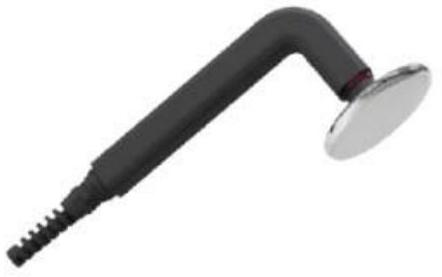
\includegraphics[max width=0.5\textwidth]{d37529a0-3e88-4d45-bc8d-f5015b8b0964-05_277_442_1722_260}
%	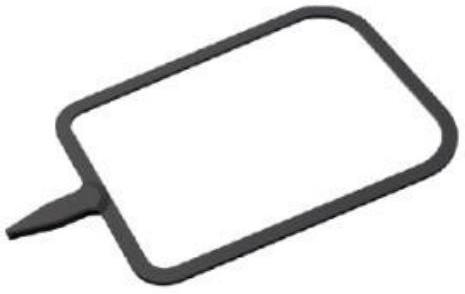
\includegraphics[max width=0.5\textwidth]{d37529a0-3e88-4d45-bc8d-f5015b8b0964-05_294_465_2270_264}
%	\caption{Manipolo resistivo}
%\end{figure}

\begin{figure}[H]
	\centering
	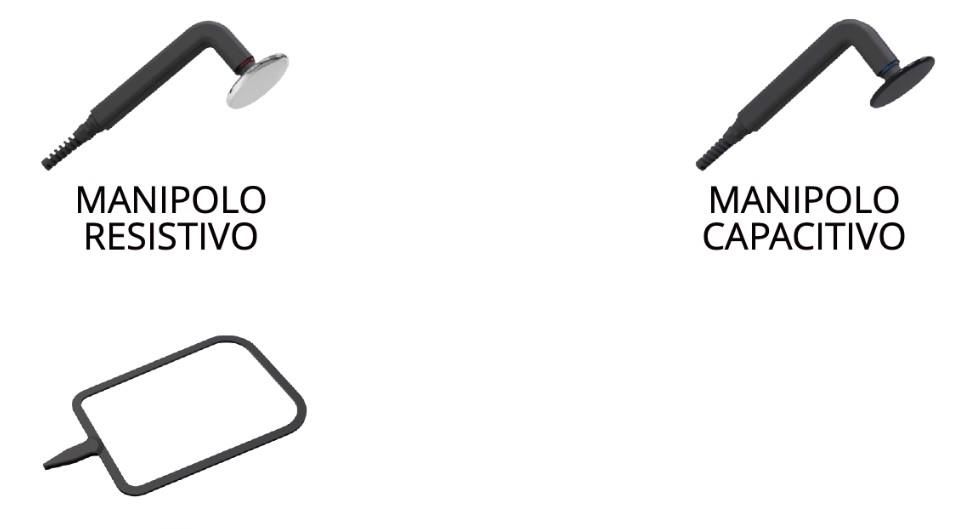
\includegraphics[max width=\textwidth]{manipolo_capacitivo}
\end{figure}


\begin{itemize}
  \item Il manipolo resistivo è particolarmente adatto per trattamenti su tessuti più profondi e densi, come muscoli e tendini.
  \item Il manipolo capacitivo, invece, è ideale per trattamenti superficiali e sui tessuti molli, come pelle e tessuto adiposo. Questa combinazione di tecnologie consente il trattamento efficace di un'ampia gamma di inestetismi, dalla lassità cutanea alla cellulite.
\end{itemize}

\subsection{Precauzioni per l'uso}

\textbf{Avvertimento} \faExclamationTriangle

\begin{itemize}
	\item Questa apparecchiatura non è adatta a pazienti affetti da ipertensione, malattie cardiache e diabete.
	\item Non adatto a donne in allattamento o durante il ciclo mestruale. Non deve essere utilizzato da pazienti con malattie infettive o tumori.
	\item Tenere i bambini lontani dal prodotto e impedire che lo trattino come un giocattolo, poiché potrebbe rappresentare un pericolo.
	\item Durante l'uso, la sonda di potenza non deve rimanere nella stessa posizione per evitare ustioni.
\end{itemize}

\vspace{20pt}

\noindent \textbf{Attenzione} \faExclamationTriangle

\begin{itemize}
  \item Prima dell'uso, verificare che il cavo di collegamento, la spina del cavo di alimentazione e la sonda siano completamente inseriti e installati.
\end{itemize}

\begin{itemize}
	\item Prima del trattamento, selezionare l'attrezzatura e la sonda appropriate.
	\item Non dedicare troppo tempo alla cura di una sola zona della pelle per evitare scottature.
	\item Dopo l'operazione di trattamento, la sonda deve essere disinfettata con alcol al 75\% e conservata correttamente in un luogo asciutto.
	\item Applicare il gel o l'essenza appropriati sulle parti del corpo per idratare la pelle.
	\item Assicurarsi che tutti gli elettrodi siano completamente a contatto con la pelle del paziente, applicando una forza moderata per evitare formicolio o macchie rosse causate dall'accumulo di corrente.
\end{itemize}

\section{Precauzioni di installazione}
\begin{itemize}
	\item Lo strumento di bellezza multifunzionale F-365 comprende una piastra negativa, due impugnature e due sonde.
	\item Le impugnature in modalità resistenza RES sono contrassegnate da un cerchio rosso e devono essere montate solo con sonde in acciaio inossidabile.
	\item L'impugnatura in modalità capacitiva CAP con logo circolare blu deve essere montata solo con una sonda nera.
	\item Le due sonde hanno perni di diametro diverso, quindi è essenziale installare correttamente la sonda corretta nell'impugnatura. Se la sonda non è installata correttamente, potrebbe allentarsi o staccarsi facilmente, rendendo difficile la regolazione.
\end{itemize}

\begin{figure}[H]
	\centering
	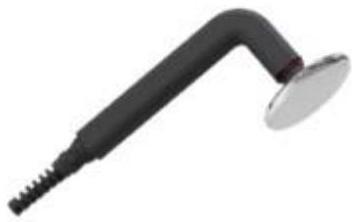
\includegraphics[width=0.5\textwidth]{d37529a0-3e88-4d45-bc8d-f5015b8b0964-07_222_359_274_187}
	\caption{Manipolo resistivo}
\end{figure}

\begin{figure}[H]
	\centering
	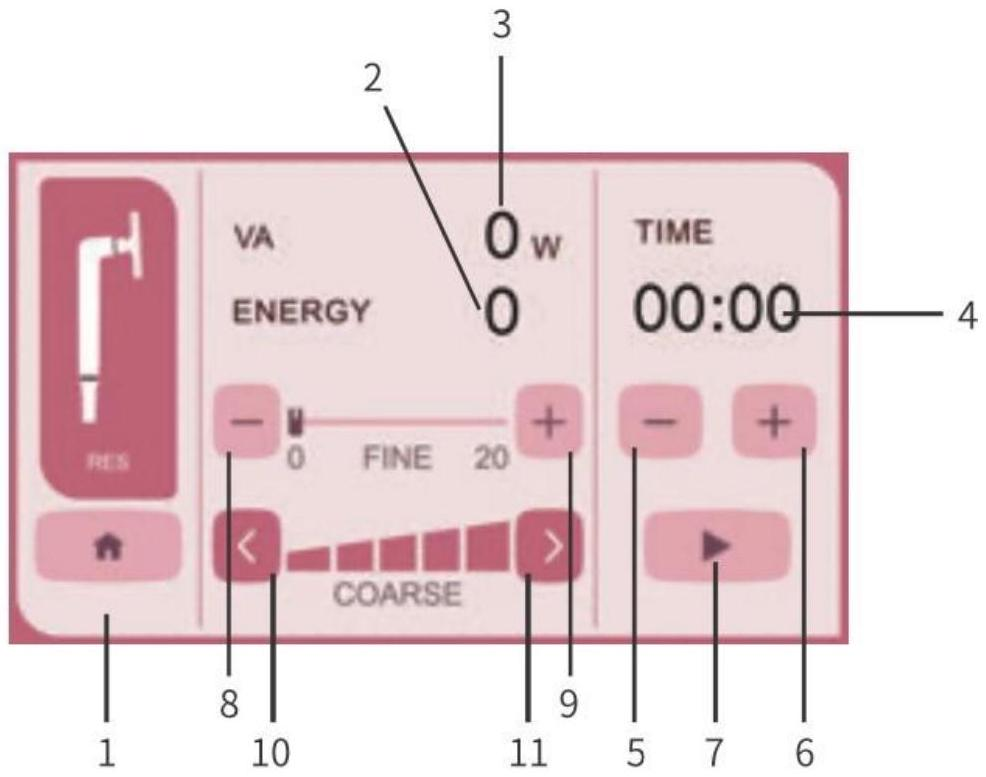
\includegraphics[width=0.7\textwidth]{d37529a0-3e88-4d45-bc8d-f5015b8b0964-07_777_986_251_826}
\end{figure}

\begin{enumerate}
  \item Torna all'interfaccia principale
  \item Visualizzazione della potenza in tempo reale. 
  \\
  L'impugnatura e la piastra negativa formano un anello che indica la potenza di uscita effettiva.
	\item Visualizzazione dell'intervallo di output: Visualizza l'intervallo impostato da 0 a 100.
	\item Visualizzazione del tempo di lavoro: Quando inizi a lavorare, il tempo di lavoro inizierà a scorrere. Quando il conto alla rovescia raggiunge lo zero, il dispositivo interrompe automaticamente l'uscita.
	\item Ridurre l'orario di lavoro: Intervallo di tempo di lavoro: 1-60 minuti.
	\item Aumentare l'orario di lavoro: Intervallo di tempo di lavoro: 1-60 minuti
	\item Avvio/Pausa
	\item L'intensità di uscita viene ridotta tramite una regolazione fine. 20 livelli regolabili
	\item L'intensità di uscita aumenta leggermente. 20 livelli regolabili.
	\item Riduzione del resto lordo. 5 livelli regolabili, ogni livello può essere regolato su 20 livelli.
	\item Aumento del cambiamento lordo. 5 livelli regolabili, ogni livello può essere regolato su 20 livelli.
\end{enumerate}

\section{Metodo di funzionamento}
Rimuovere la maniglia e installare la sonda in acciaio inossidabile.\\
Dopo che il paziente ha toccato la piastra negativa, premere il pulsante di avvio per avviare la funzione. Una volta trascorso il tempo, le sonde smetteranno di funzionare. Rimuovere la sonda, pulirla e riposizionare l'impugnatura e la sonda nel supporto accessori.

\begin{figure}[H]
	\centering
	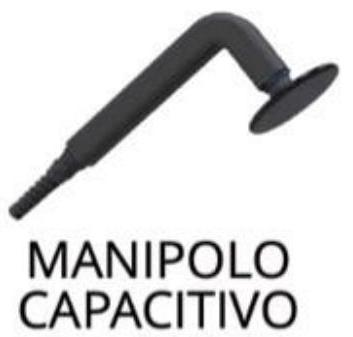
\includegraphics[width=0.5\textwidth]{d37529a0-3e88-4d45-bc8d-f5015b8b0964-08_337_353_520_139}
\end{figure}

\begin{figure}[H]
	\centering
	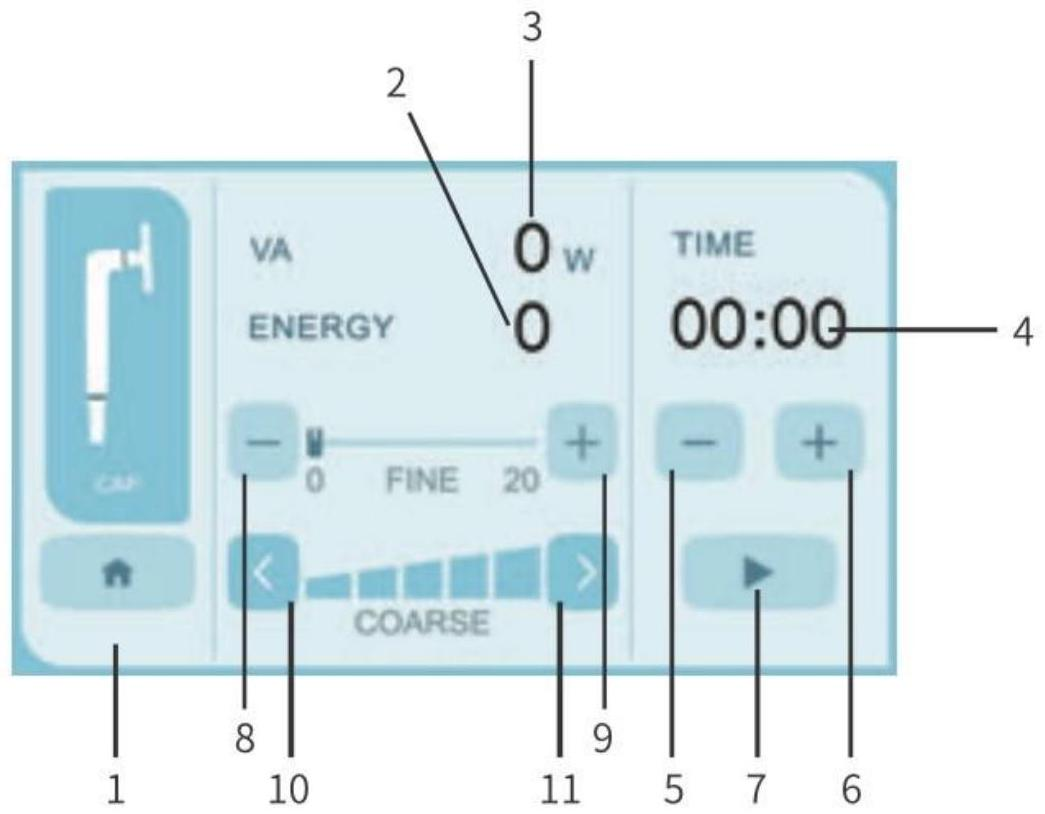
\includegraphics[width=0.8\textwidth]{d37529a0-3e88-4d45-bc8d-f5015b8b0964-08_814_1045_516_829}
\end{figure}

\begin{enumerate}
  \item Torna all'interfaccia principale.
  \item Visualizzazione della potenza in tempo reale: l'impugnatura e la piastra negativa formano un anello per mostrare la potenza di uscita effettiva.
  \item Visualizzazione dell'intervallo di uscita, mostra l'intervallo impostato da 0 a 100.
  \item Visualizzazione del tempo di lavoro: quando inizi a lavorare, il tempo di lavoro inizierà il conto alla rovescia.\\
  Quando il conto alla rovescia raggiunge lo zero, il dispositivo interrompe automaticamente l'uscita.
  \item Ridurre il tempo di lavoro, intervallo di tempo di lavoro: 1-60 minuti.
  \item Aumentare il tempo di lavoro, intervallo di tempo di lavoro: 1-60 minuti.
  \item Avvio/Pausa.
  \item L'intensità di uscita viene ridotta tramite una regolazione fine, 20 velocità regolabili.
  \item L'intensità di uscita aumenta leggermente, con 20 livelli regolabili.
  \item Resto lordo ridotto, 5 livelli regolabili, ogni livello può essere regolato in 20 livelli.
  \item Aumento del cambiamento lordo, 5 livelli regolabili, ogni livello può essere regolato su 20 livelli.
\end{enumerate}

\section{Metodo di funzionamento}
\begin{enumerate}
  \item Regolare la fasatura e l'ingranaggio di uscita;
  \item Rimuovere la maniglia e installare la sonda nera.
  \item Dopo che i clienti hanno toccato la piastra negativa, premere il pulsante di avvio per avviare la funzione;
  \item Una volta trascorso il tempo, l'accessorio smetterà di funzionare. Rimuovere la sonda, quindi pulirla e riposizionare l'impugnatura e la sonda sul ripiano degli accessori.
  \item Apparecchiatura all'avanguardia per trattamenti corpo a radiofrequenza. Si tratta di un dispositivo professionale per trattamenti a radiofrequenza, progettato per offrire risultati eccellenti nel campo dell'estetica.
\end{enumerate}

Grazie al suo design innovativo e alle sue funzionalità avanzate, rappresenta una soluzione versatile e potente per il ringiovanimento della pelle, il trattamento delle rughe, la tonificazione e la riduzione delle imperfezioni della pelle.

\section{Touchscreen intuitivo}
\begin{enumerate}
	\item Il dispositivo è dotato di un touch screen che consente una visualizzazione e un controllo semplici e intuitivi di tutti i parametri.
	\\
	Questo sistema consente agli operatori di gestire il trattamento con precisione, garantendo il massimo comfort del paziente e risultati ottimali.
	\item Con 20 livelli di intensità regolabili, questo dispositivo offre una personalizzazione completa dell' trattamento. La potenza può essere regolata in base alle specifiche esigenze del paziente, garantendo una soluzione specifica per ogni tipo di pelle e condizione estetica.
	\item Offre due modalità operative con diverse forme d'onda: continua e pulsata. La modalità continua è ideale per trattamenti più profondi e intensi, mentre la modalità pulsata è perfetta per procedure più delicate o aree sensibili, offrendo una versatilità senza pari.
	\item Manipoli resistivi e capacitivi, il dispositivo è dotato di due impugnature manuali: una resistiva e una capacitiva.
	\item Sonda e piastra elettrodo negativa: include una sonda di precisione e una piastra elettrodo negativa che lavorano in sinergia per garantire una distribuzione uniforme dell'energia e una conduzione efficiente delle onde radio nel tessuto. Ciò garantisce trattamenti sicuri ed efficaci.
	\item Tempo di lavoro regolabile, il dispositivo consente di regolare il tempo di lavoro da 1 a 60 minuti. offrendo la possibilità di personalizzare la durata del trattamento in base alle specifiche esigenze del paziente e al tipo di trattamento richiesto.
\end{enumerate}

\section{Benefici dei trattamenti}
\begin{itemize}
  \item Efficacia e sicurezza: La radiofrequenza è una tecnologia ampiamente utilizzata in campo estetico per stimolare la produzione di collagene e migliorare l'elasticità della pelle, senza procedure invasive.
  \item Versatilità: Grazie ai manipoli resistivi e capacitivi, è adatto al trattamento di un'ampia gamma di inestetismi, dalle rughe alla cellulite, garantendo risultati visibili in poche sedute.
  \item Controllo totale: il touch screen e i numerosi parametri regolabili rendono l'utilizzo dell'attrezzatura estremamente semplice e preciso, per un'esperienza utente professionale e performante.
\end{itemize}

\section{Principali applicazioni}
\begin{itemize}
  \item Ringiovanimento della pelle: stimola la produzione di collagene e favorisce un effetto lifting naturale.
  \item Riduzione delle rughe: Grazie al riscaldamento controllato dei tessuti, favorisce la levigatura delle linee sottili e rughe profonde.
  \item Tonificazione della pelle: rende la pelle più soda e tonica, riducendo il rilassamento cutaneo.
  \item Trattamento anticellulite: agisce in profondità nel tessuto adiposo, favorendo il drenaggio liquidi e migliorando l'aspetto della pelle a buccia d'arancia.
\end{itemize}

\section{Manutenzione e risoluzione dei problemi}
Il sistema può funzionare correttamente solo se sono soddisfatte tutte le seguenti condizioni:

\begin{itemize}
  \item Il personale ha rispettato tutte le norme di sicurezza.
  \item Il personale ha letto il manuale utente.
  \item Il dispositivo è collegato correttamente alla presa di corrente.
  \item Interruttore situato nella parte posteriore in posizione ON.
\end{itemize}

%\begin{center}
%\begin{tabular}{|l|l|l|}
%\hline
%Tipo di guasto & Motivo & Soluzione \\
%\hline
%Il dispositivo non funziona o si blocca & \begin{tabular}{l}
%1. Nessuna alimentazione \\
%2. Il cavo di alimentazione non è collegato correttamente \\
%Collegato o inserito correttamente \\
%\end{tabular} & \begin{tabular}{l}
%1. Controllare se il fusibile si trova nella scatola dei fusibili alla base \\
%L'alimentatore è bruciato. \\
%Se \\
%Se il fusibile è bruciato, sostituire il fusibile corrispondente con uno nuovo. \\
%2. Premere il pulsante di avvio; il pulsante si illuminerà dopo l'accensione. \\
%\end{tabular} \\
%\hline
%Lo schermo non funziona. & 1 Senza alimentazione & 2. Collegare o inserire il cavo di alimentazione correttamente. \\
%\hline
%La sonda associata non funziona & Scarso contatto dell'interfaccia & 1. Accendere l'alimentazione. \\
%\hline
%\end{tabular}
%\end{center}

%
	\begin{table}[H]
		\centering
		\renewcommand{\arraystretch}{1.3} % aumenta leggermente l'altezza delle righe
		\begin{tabularx}{\textwidth}{|p{3cm}|>{\raggedright\arraybackslash}X|>{\raggedright\arraybackslash}X|}
			\hline
			\textbf{Tipo di guasto} & \textbf{Motivo} & \textbf{Soluzione} \\
			\hline
			Il dispositivo non funziona o si blocca & 
			1. Nessuna alimentazione \newline
			2. Il cavo di alimentazione non è collegato/inserito correttamente & 
			1. Controllare se il fusibile si trova nella scatola dei fusibili alla base \newline
			L'alimentatore è bruciato. \newline
			Se \newline
			Se il fusibile è bruciato, sostituire il fusibile corrispondente con uno nuovo. \newline
			2. Premere il pulsante di avvio; il pulsante si illuminerà dopo l'accensione. \\
			\hline
			Lo schermo non funziona. & 
			1 Senza alimentazione & 
			2. Collegare o inserire il cavo di alimentazione correttamente. \\
			\hline
			La sonda associata non funziona & 
			Scarso contatto dell'interfaccia & 
			1. Accendere l'alimentazione. \\
			\hline
		\end{tabularx}
	\end{table}
%

\section{Contenuto:}
\begin{center}
\begin{tabular}{|l|l|}
\hline
Tensione / Frequenza & CA $100-120 \mathrm{~V}, 50 / 960 \mathrm{~Hz}$ : CA $220-240 \mathrm{~V}, 50 / 60 \mathrm{~Hz}$ \\
\hline
Energia & 400 W \\
\hline
Peso & $6,8 \mathrm{~kg}$ \\
\hline
Dimensioni del prodotto & $37 \times 31 \times 16,5$ centimetri \\
\hline
Dimensioni dell'imballaggio & Dispositivi $\times$ 1 \\
\hline
Contenuto della confezione & Accessori x1 \\
\hline
 & Manipolatore capacitivo $\times$1 \\
\hline
 & Maniglia resistiva $\times$ 1 \\
\hline
 & Lastra negativa \\
\hline
 & Elettrodi $\times$ 8 \\
\hline
 & Cacciavite \\
\hline
 & Viti M4 $\times$ 2 \\
\hline
 & Manuale \\
\hline
 & Cavo di alimentazione \\
\hline
\end{tabular}
\end{center}

\section{CONSENSO INFORMATO - Trattamento estetico "RF-USION POWER+"}
\subsection{DATI CLIENTE}
Nome e Cognome: $\_\_\_\_$\\
Data di nascita: $\_\_\_\_$\\
Telefono: $\_\_\_\_$

\subsection{DATI OPERATORE / CENTRO}
Nome centro: $\_\_\_\_$\\
Operatore: $\_\_\_\_$

\subsection{DESCRIZIONE DEL TRATTAMENTO}
Il trattamento RF-USION POWER+ utilizza tecnologia a radiofrequenza per stimolare i tessuti cutanei in profondità, favorire la produzione di collagene ed elastina, migliorare la tonicità della pelle e contrastare lassità cutanee.

\subsection{POSSIBILI EFFETTI}
Lieve arrossamento temporaneo, sensazione di calore, lieve edema o sensibilità nella zona trattata.

\subsection{CONTROINDICAZIONI}
Gravidanza, pacemaker o dispositivi elettronici impiantati, patologie cardiache importanti, epilessia, patologie oncologiche in corso, infezioni o infiammazioni nella zona trattata, presenza di protesi metalliche nella zona (se rilevante).

\subsection{DICHIARAZIONI DEL CLIENTE}
Dichiaro di aver ricevuto spiegazioni chiare, di essere a conoscenza che si tratta di trattamento estetico e non medico, e di autorizzare l'esecuzione del trattamento.

\subsection{PRIVACY}
I dati saranno trattati nel rispetto del Regolamento UE 2016/679 (GDPR).\\
Firma Cliente: $\_\_\_\_$\\
Firma Operatore: $\_\_\_\_$\\
Data: $\_\_\_\_$ 1 $\_\_\_\_$ $/$ $\_\_\_\_$

% --- INIZIO INFORMATIVA PRIVACY ---
\newpage

\section{INFORMATIVA PRIVACY}
\begin{center}
	(ai sensi dell'art. 13 del Regolamento UE 2016/679)
\end{center}

La presente informativa è resa ai sensi del Regolamento Generale sulla Protezione dei Dati (GDPR) e riguarda il trattamento dei dati personali dei clienti che si sottopongono a trattamenti e tecnologie estetiche.

\subsection*{Titolare del trattamento}

Il Titolare del trattamento è:

\begin{itemize}
	\item Denominazione centro estetico: \underline{\hspace{5cm}}
	\item Sede legale: \underline{\hspace{7cm}}
	\item P. IVA / C.F.: \underline{\hspace{6cm}}
	\item Contatti (telefono/email): \underline{\hspace{5cm}}
\end{itemize}

\subsection*{Tipologia di dati trattati}

Il Titolare può raccogliere e trattare le seguenti categorie di dati:

\begin{itemize}
	\item Dati anagrafici (nome, cognome, data di nascita)
	\item Dati di contatto (telefono, e-mail)
	\item Dati fiscali per eventuale fatturazione
	\item Dati particolari relativi allo stato di salute (allergie, patologie, gravidanza, terapie in corso) necessari per valutare l'idoneità ai trattamenti estetici
	\item Eventuali immagini fotografiche prima/dopo trattamento (previo consenso specifico)
\end{itemize}

\subsection*{Finalità del trattamento}

I dati personali sono trattati per le seguenti finalità:

\begin{enumerate}
	\item Esecuzione di trattamenti estetici e utilizzo di tecnologie professionali (laser, radiofrequenza, ultrasuoni, pressoterapia, ecc.)
	\item Valutazione dell'idoneità al trattamento
	\item Adempimenti amministrativi, contabili e fiscali
	\item Gestione degli appuntamenti
	\item Eventuale invio di comunicazioni promozionali (solo previo consenso separato)
	\item Eventuale utilizzo di immagini per finalità informative o promozionali (solo previo consenso separato)
\end{enumerate}

\subsection*{Base giuridica del trattamento}

Il trattamento dei dati si fonda su:

\begin{itemize}
	\item Esecuzione del contratto/prestazione richiesta
	\item Adempimento di obblighi di legge
	\item Consenso esplicito dell'interessato per il trattamento di dati particolari (sanitari)
	\item Consenso separato per marketing e utilizzo immagini
\end{itemize}

\subsection*{Modalità di trattamento}

Il trattamento dei dati avviene mediante strumenti cartacei e/o informatici, nel rispetto dei principi di correttezza, liceità, trasparenza e tutela della riservatezza.

Sono adottate adeguate misure di sicurezza per prevenire accessi non autorizzati, perdita o diffusione dei dati.

\subsection*{Conservazione dei dati}

I dati personali saranno conservati:

\begin{itemize}
	\item Per il tempo necessario all'erogazione del servizio
	\item Per il periodo previsto dalla normativa fiscale e civilistica
	\item Fino a revoca del consenso per finalità di marketing o utilizzo immagini
\end{itemize}

\subsection*{Comunicazione dei dati}

I dati potranno essere comunicati a:

\begin{itemize}
	\item Consulenti fiscali e amministrativi
	\item Software gestionali utilizzati per la gestione clienti
	\item Autorità competenti, ove previsto dalla legge
\end{itemize}

I dati non saranno diffusi senza consenso.

\subsection*{Diritti dell'interessato}

L'interessato può esercitare in qualsiasi momento i seguenti diritti:

\begin{itemize}
	\item Accesso ai propri dati
	\item Rettifica o aggiornamento
	\item Cancellazione (diritto all'oblio)
	\item Limitazione del trattamento
	\item Opposizione al trattamento
	\item Revoca del consenso
	\item Reclamo all'Autorità Garante per la Protezione dei Dati Personali
\end{itemize}

Le richieste possono essere inviate ai recapiti del Titolare sopra indicati.

\subsection*{Natura del conferimento dei dati}

Il conferimento dei dati è necessario per l'erogazione dei trattamenti estetici.
Il mancato conferimento può comportare l'impossibilità di eseguire il servizio.

\subsection*{CONSENSO}

Il/La sottoscritto/a dichiara di aver ricevuto e compreso la presente informativa.

\vspace{0.8cm}

Data: \underline{\hspace{5cm}} 

\vspace{15pt}
Firma: \underline{\hspace{6cm}}

\vspace{1cm}

$\square$ Acconsento al trattamento dei dati particolari (sanitari)

\vspace{0.3cm}
$\square$ Acconsento all'utilizzo delle immagini per finalità promozionali

\vspace{0.3cm}
$\square$ Acconsento a ricevere comunicazioni promozionali

% --- FINE INFORMATIVA PRIVACY ---

\newpage


\begin{figure}[H]
	\centering
	\includegraphics[width=0.7\paperwidth,height=\paperheight, keepaspectratio]{"../cose da aggiungere/privacy_conformita/dichiarazione_conformita"}
\end{figure}


\end{document}